\documentclass[12pt,a4paper]{article}
\usepackage{graphicx}
\usepackage{multicol}
\usepackage[margin=1in]{geometry}
\usepackage{titlesec}
\titleformat*{\section}{\large\bfseries}
\titleformat*{\subsection}{\bfseries}
\begin{document}
\begin{center}
{\LARGE \textbf{mdpd}}\\
{\large (Extending Markdown to Embed Puredata Patches)}\\
\vspace{1em}
{\normalsize Ryoma Okuda (s1270174), Supervisor: Prof. Julián Villegas}\\
\end{center}
\begin{multicols}{2}
\section*{1. Motivation and Goal}
\subsection*{1.1 Motivation}
The ability to easily integrate and display dynamic content like PureData within a commonly used markup language like markdown has benefits for users in the audio programming. Also my professor wanted this functionality for their class.
\subsection*{1.2 Goal}
As we extend PureData, we need to make sure existing functionality still works. This includes ensuring that all functions implemented in original PureData continue to operate as we expected.
\section*{2. Approach/Methodology}
We started by selecting NodeJS and WebPD for the project. Using these tools, we developed a compiler that can interpret both the content in Markdown and the patches from Puredata. 
The goal was to integrate PureData code within a Markdown environment.
\section*{3. Current Results and Status}
We've successfully implemented an mdpd to HTML previewer. 

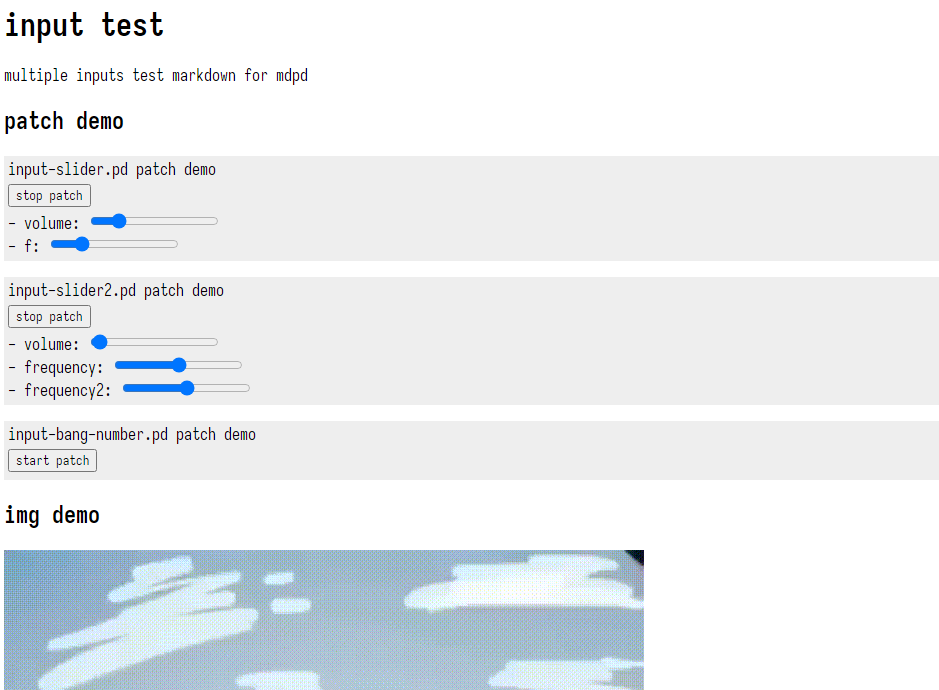
\includegraphics[width=0.5\linewidth]{mdpd_ss.png}
\\ \textit{mdpd previewer}


This allows users to view their Markdown and PureData content directly in a web browser.
The next step is to develop an mdpd to PDF converter, which will enable users to save and share their creations in accessible format. 
\end{multicols}
\end{document}

